\documentclass{beamer}
%\usepackage[T1]{fontenc}
\usepackage[utf8]{inputenc}
%\usepackage{lmodern}  % Use the Latin Modern font family

\usepackage{latexsym,amsmath, xcolor, bm, amssymb, color, tikz, graphicx, amsthm, mathtools}
\usepackage{algorithm}
\usepackage{algorithmic}
\usepackage{hyperref}
\usepackage{float}     
\usepackage{CJKutf8}
\usepackage{multicol}

\usepackage{tikz}
%\usetikzlibrary{timeline}

\DeclareMathOperator*{\argmax}{arg\,max}
\DeclareMathOperator*{\argmin}{arg\,min}
\DeclareMathOperator{\sign}{sign}
\DeclareMathOperator{\Tr}{Tr}

\makeatletter
\DeclareRobustCommand\onedot{\futurelet\@let@token\@onedot}
\def\@onedot{\ifx\@let@token.\else.\null\fi\xspace}
\def\eg{\emph{e.g}\onedot} 
\def\Eg{\emph{E.g}\onedot}
\def\ie{\emph{i.e}\onedot} 
\def\Ie{\emph{I.e}\onedot}
\def\cf{\emph{c.f}\onedot} 
\def\Cf{\emph{C.f}\onedot}
\def\etc{\emph{etc}\onedot} 
\def\vs{\emph{vs}\onedot}
\def\wrt{w.r.t\onedot} 
\def\dof{d.o.f\onedot}
\def\etal{\emph{et al}\onedot}
\makeatother


\usetheme{Madrid}
\useinnertheme{circles}

\definecolor{ColorUNR}{HTML}{990077} 
\usecolortheme[named=ColorUNR]{structure}
%\usecolortheme[named=ColorUNR]{exampleblock}

%\setbeamertemplate{blocks}[rounded][shadow=true]
%\setbeamercolor{block body}{fg=black,bg=white}



%------------------------------------------------------------
%This block of code defines the information to appear in the
%Title page
\title %optional
{Bienvenidos al Training Camp 2024}

%\subtitle{(Subtitulo de la Clase)}

%\subtitle{with applications to persuation and lie production}
% \author % (optional)
% {Author Name}

%\author[Matias Ramos]{Matias Ramos}

\institute[]{Universidad Nacional de Rosario - Facultad de Ciencias Exactas, Ingeniería y Agrimensura}
\date[TC 2024]{Training Camp 2024}
\titlegraphic{
\includegraphics[clip,height=2cm,keepaspectratio]{logos/tcarg.jpeg}}

%End of title page configuration block
%------------------------------------------------------------


%------------------------------------------------------------
%The next block of commands puts the table of contents at the 
%beginning of each section and highlights the current section:
\AtBeginSection[]
{
  \begin{frame}
    \frametitle{Temario}
    \tableofcontents[currentsection]
  \end{frame}
}
%------------------------------------------------------------


\begin{document}


%The next statement creates the title page.
\frame{\titlepage}


%------------------------------------------------------------
% Frame de Sponsors, me parece mejor ponerlo al principio
% Antes del índice/contenido

\begin{frame}{Gracias Sponsors!}
    \begin{columns}[t]
        \column{0.5\textwidth}
        \centering
        Organizador\\
        \vspace{0.8cm}
        
\includegraphics[width=0.7\textwidth,keepaspectratio]{logos/UNRlogo.png}
        
\includegraphics[width=0.7\textwidth,keepaspectratio]{logos/FCEIA.png}
        \column{0.5\textwidth}
        \centering
        Diamond\\
        
\includegraphics[width=1\textwidth,keepaspectratio]{logos/GTSlogo.jpeg}
    \end{columns}
    \begin{columns}[t]
        \column{1.0\textwidth}
        \centering
        Gold\\
        \begin{minipage}{0.5\textwidth}
            \centering
            
\includegraphics[width=0.4\textwidth,keepaspectratio]{logos/avature.jpg}
        \end{minipage}%
        \begin{minipage}{0.5\textwidth}
            \centering
            
\includegraphics[width=0.4\textwidth,keepaspectratio]{logos/Acc_Logo_Black_Purple_RGB.png}
        \end{minipage}
    \end{columns}
\end{frame}


%---------------------------------------------------------
%This block of code is for the table of contents after
%the title page
\begin{frame}
\frametitle{Temario}
\tableofcontents
\end{frame}
%---------------------------------------------------------


\section{Que es el Training Camp?}

\begin{frame}{¿Qué es el Training Camp?}
Es un entrenamiento intensivo de Programación Competitiva de 2 semanas
\begin{itemize}
    \item Teórico (módulos durante la mañana) 
    \item Práctico (simulaciones durante la tarde)
\end{itemize}
Entrenamos para prepararnos para las competecias de ICPC.
    \centering
    
\includegraphics[clip,height=3.5cm,keepaspectratio]{logos/icpc.jpeg}
\end{frame}


\tikzstyle{descript} = [text = black,align=center, minimum height=1.8cm, align=center, outer sep=0pt,font = \footnotesize]
\tikzstyle{activity} =[align=center,outer sep=1pt]

\section{El Camino de ICPC}

\begin{frame}{El Camino de ICPC}
    \centering
    
\includegraphics[clip,height=3.5cm,keepaspectratio]{logos/icpc.jpeg}

    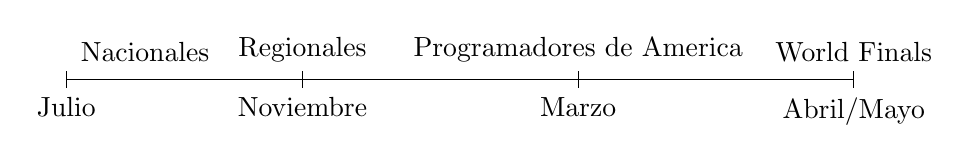
\begin{tikzpicture}
        \draw (1,0) -- (11,0);
        \foreach \x in {1,4,7.5,11}
            \draw (\x cm,3pt) -- (\x cm,-3pt);
            \draw (1,0) node[below=3pt] {Julio} node[above=3pt] {};
            \draw (2,0) node[below=3pt] {} node[above=3pt] {Nacionales};
            \draw (4,0) node[below=3pt] {Noviembre} node[above=3pt] {Regionales};
            \draw (7.5,0) node[below=3pt] {Marzo} node[above=3pt] {Programadores de America};
            \draw (11,0) node[below=3pt] {Abril/Mayo} node[above=3pt] {World Finals};
    \end{tikzpicture}
\end{frame}

\section{Cronograma}


\begin{frame}{Día Inaugural}
    Usted está aquí
    \centering
    \includegraphics[clip,height=7cm,keepaspectratio]{img/00_inaugu.png}
\end{frame}

\begin{frame}{Almuerzo}
    \centering
    El almuerzo es de {\bf 12 a 13 hs}, el horario se respeta siempre.
    
    {\bf No lleguen tarde.}
\end{frame}


\begin{frame}{Día GTS}
    \centering
    \includegraphics[clip,height=4.5cm,keepaspectratio]{img/01_gts.png}
\end{frame}

\begin{frame}{Días normales}
    \centering
    \includegraphics[clip,height=7cm,keepaspectratio]{img/02_normal.png}
\end{frame}


\begin{frame}{Días Sponsors Gold}
    \centering
    \includegraphics[clip,height=7cm,keepaspectratio]{img/03_gold.png}
\end{frame}


\begin{frame}{Día de Cierre}
    \centering
    \includegraphics[clip,height=7cm,keepaspectratio]{img/04_cierre.png}
\end{frame}

\begin{frame}{Dudas}
Para dudas o consultas pueden:
        \begin{itemize}
            \item Contactar al Staff (voluntarios u organizadores)
            \item Preguntar por el grupo de Telegram
        \end{itemize}
        %\bibliography{ref}
\end{frame}


\end{document}
